\documentclass[10pt, a4paper, ngerman]{arbeitsblatt}

\ladeModule{theme}

\ladeFach[quelltexte]{informatik}

\aboptionen{
	name		= {J. Neugebauer},
	kuerzel 	= {Ngb},
	titel 		= {Klausurvorbereitung},
	reihe 		= {Lineare Datenstrukturen},
	fach 		= {Informatik},
	kurs 		= {Q1},
	nummer 		= {II.9},
	lizenz 		= {cc-by-nc-sa-eu-4},
	version 	= {2022-11-14},
}

\begin{document}
\ReiheTitel

\begin{aufgabe}
Analysiere den gezeigten Quelltext und beschreibe seine Funktionsweise.

\begin{minted}{java}
public int tueEtwas ( List<Integer> pList ) {
	int a = Integer.MAX_VALUE;

	pList.toFirst();
	while( pList.hasAccess() ) {
		if ( pList.getContent() < a ) {
			a = pList. getContent();
		}
		pList.next();
	}
	return a;
}
\end{minted}
\end{aufgabe}


\begin{aufgabe}
Erweitere die generische Klasse List um eine Methode \mintinline{java}{concat(Queue<ContentType> pQueue)}, die alle Elemente einer Schlange an die Liste anhängt.
\end{aufgabe}

\begin{aufgabe}
	\begin{wrapfix}
	\begin{wrapfigure}[8]{r}{0pt}
		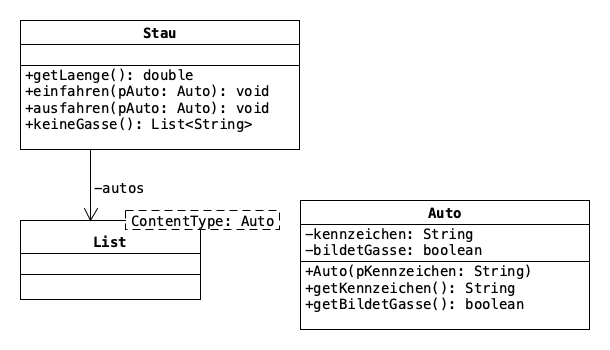
\includegraphics[width=7cm]{Q1-AB.II.09-CD_Stau.png}
	\end{wrapfigure}

Das Implementierungsklassendiagramm zeigt einen Ausschnitt aus der Modellierung einer Verkehrsüberwachung. Das Programm kann sich bildende Staus überwachen und über Kameras feststellen, ob die Autos eine Rettungsgasse bilden. Außerdem kann das Kennzeichen der PKW eingelesen werden.

Implementiere die Methode \mintinline{java}{keineGasse()}, die aus der Liste der wartenden Autos die Kennzeichen derjenigen ermittelt, die keine Rettungsgasse bilden.
\end{wrapfix}
\end{aufgabe}

\begin{aufgabe}
Ein Bowlingcenter hat sechs Bowlingbahnen. Zu jeder Bahn gehört eine Rinne, in die die gespielten Kugeln zurückbefördert werden. Von der Rinne aus kann ein Spieler dann die gewünschte Kugel nehmen. Die Kugeln haben unterschiedliche Gewichte und dazu jeweils eine passende Farbe.

\begin{enuma}
	\item Für die Rinne bieten sich die Datenstrukturen der Schlange und der Liste an. \operator{Begründe} die Wahl der Liste in Abgrenzung zur Schlange.

	\item\label{taufg:bowling-sorten} \operator{Implementiere} den Konstruktor der Klasse Kugel so, dass die Gewichts- und Farbkombination nicht beliebig sein kann. Eine 10-kg-Kugel muss also die Farbe Blau haben, eine 8-kg-Kugel die Farbe Gelb und eine 6-kg-Kugel die Farbe Rosa. (Es kann hier davon ausgegangen werden, dass es nur diese drei Farb-Gewichts-Kombinationen gibt.)

	\item In der Rinne können blaue, gelbe oder rosa Kugeln liegen.

	\operator{Entwickele} eine Strategie, mit der die in einer Rinne am häufigsten vertretene Farbe identifiziert und ausgegeben werden kann. Sollten zwei Farben gleich häufig vorkommen, wird diejenige mit dem höchsten Gewicht (siehe \prettyref{taufg:bowling-sorten}) ausgegeben.

	\operator{Implementiere} die entsprechende Methode \mintinline{java}{public String haeufigsteFarbe()} der Klasse Rinne.

	\item
	Zwischen je zwei Bahnen gibt es noch Kugelständer mit 20 Plätzen für Kugeln. Es gibt also fünf solcher Kugelständer. Die Verwaltung der Kugeln im Kugelständer läuft über ein Array \code{vorrat}. Die Klasse \code{Spieler} kennt die Klasse \code{Kugelständer}. In dem Array \code{pStaender} sind die fünf Ständer gespeichert.

	\begin{center}
		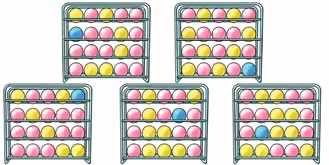
\includegraphics[width=6cm]{Q1-AB.II.09-Abb_Bowlingstaender.png}
	\end{center}

	\operator{Analysiere} die folgende Methode der Klasse \code{Spieler}. \operator{Gib} für das Beispiel in der Abbildung die Belegung der fünf Ständer \operator{an}, nachdem die Methode ausgeführt wurde.

	\begin{minted}{java}
	public void methode1( Staender[] pStaender ) {
		for(int a=0; a < 100; a++) {
			for(int i=0; i < pStaender.length; i++) {
				for (int j=0; j < 20; j++) {
					Kugel aktKugel = pStaender[i].vorrat[j];
					if(aktKugel.getFarbe().equals("blau")) {
						if(j < 19) {
							Kugel hilf = aktKugel;
							pStaender[i].vorrat[j] = pStaender[i].vorrat[j+1];
							pStaender[i].vorrat[j+1] = hilf;
						} else if(i < pStaender.length - 1) {
							Kugel hilf = aktKugel;
							pStaender[i].vorrat[j] = pStaender[i+1].vorrat[0];
							pStaender[i+1].vorrat[0] = aktKugel;
						}
					}
				}
			}
		}
	}
	\end{minted}
\end{enuma}
\end{aufgabe}
\end{document}
